\chapter{Teoretická část}
% udělat popisek teoretické části, metody, co tam máme všechno.
Tato kapitola shrnuje teoretická východiska a klíčové metody potřebné pro návrh a realizaci automatizovaného systému dopravního monitoringu. V~úvodních sekcích jsou rozebrány principy víceobjektového sledování (\acs{MOT}), stavové predikce pomocí Kalmanova filtru a prostorové metody sčítání průjezdů využívající oblasti zájmu (\acs{ROI}). Navazující část se věnuje předzpracování obrazových dat a evoluci hlubokých konvolučních neuronových sítí (\acs{CNN}) pro jednofázovou detekci objektů v~reálném čase, přičemž hlavní důraz je kladen na architekturu rodiny \acs{YOLO} a porovnání jejích velikostních variant. Závěr kapitoly zasazuje tyto algoritmy do kontextu moderních inteligentních dopravních systémů, vysvětluje principy výpočtů na okraji sítě (\acs{Edge AI}) s~využitím hardwarových akcelerátorů (\acs{NPU}), definuje exaktní matematické metriky pro evaluaci přesnosti a vymezuje legislativní požadavky ochrany soukromí dle nařízení \acs{GDPR}.

\section{Sledování a počítání objektů}
Sledování objektů v~obrazových sekvencích a videu představuje klíčovou nadstavbu nad samotnou detekcí objektů. Zatímco detekce umožňuje lokalizovat a klasifikovat objekty v~jednotlivých izolovaných snímcích, sledování zajišťuje jejich konzistentní identifikaci napříč časem. Tato vlastnost je vysoce heterogenní a zásadní zejména v~dopravních aplikacích, kde je pro komplexní analýzu nutné sledovat plynulý pohyb vozidel, určovat jejich trajektorie, rychlost nebo měřit přesný počet průjezdů daným úsekem komunikace~\cite{szeliski_computer_vision, zhou_traffic_survey_2024}.

\subsection{Víceobjektové sledování (MOT)}
Víceobjektové sledování (\acs{MOT}, z~angl. \textit{Multiple Object Tracking}) se zabývá současným sledováním většího počtu dynamických objektů ve scéně. Hlavním cílem je přiřazení unikátních a časově konzistentních identifikátorů (Unique \acs{ID}) každému objektu při jeho prvním výskytu ve scéně. Tento identifikátor je následně udržován po celou dobu výskytu entity ve sledované sekvenci, což umožňuje spojování detekcí mezi jednotlivými snímky a rekonstrukci trajektorie objektu v~čase. V~dopravních monitorovacích systémech nachází \acs{MOT} uplatnění zejména při analýze dopravních toků, odhadu hustoty provozu, detekci anomálií nebo sledování pohybu vozidel a chodců na komplexních křižovatkách~\cite{zhou_traffic_survey_2024}.

Tento proces je ve většině moderních architektur realizován pomocí přístupu „detekce před sledováním“ (z~angl. \textit{Tracking-by-Detection}). Systém nejprve v~každém snímku identifikuje objekty pomocí detekčního konvolučního modelu a následně provádí asociaci těchto detekcí mezi po sobě jdoucími snímky na základě kombinace prostorových, časových a vzhledových charakteristik. Správná správa těchto identifikátorů je kritická pro následné navazující úlohy, jako je statistické počítání objektů nebo pokročilá analýza jejich chování~\cite{szeliski_computer_vision}.

\begin{figure}[H]
    \centering
    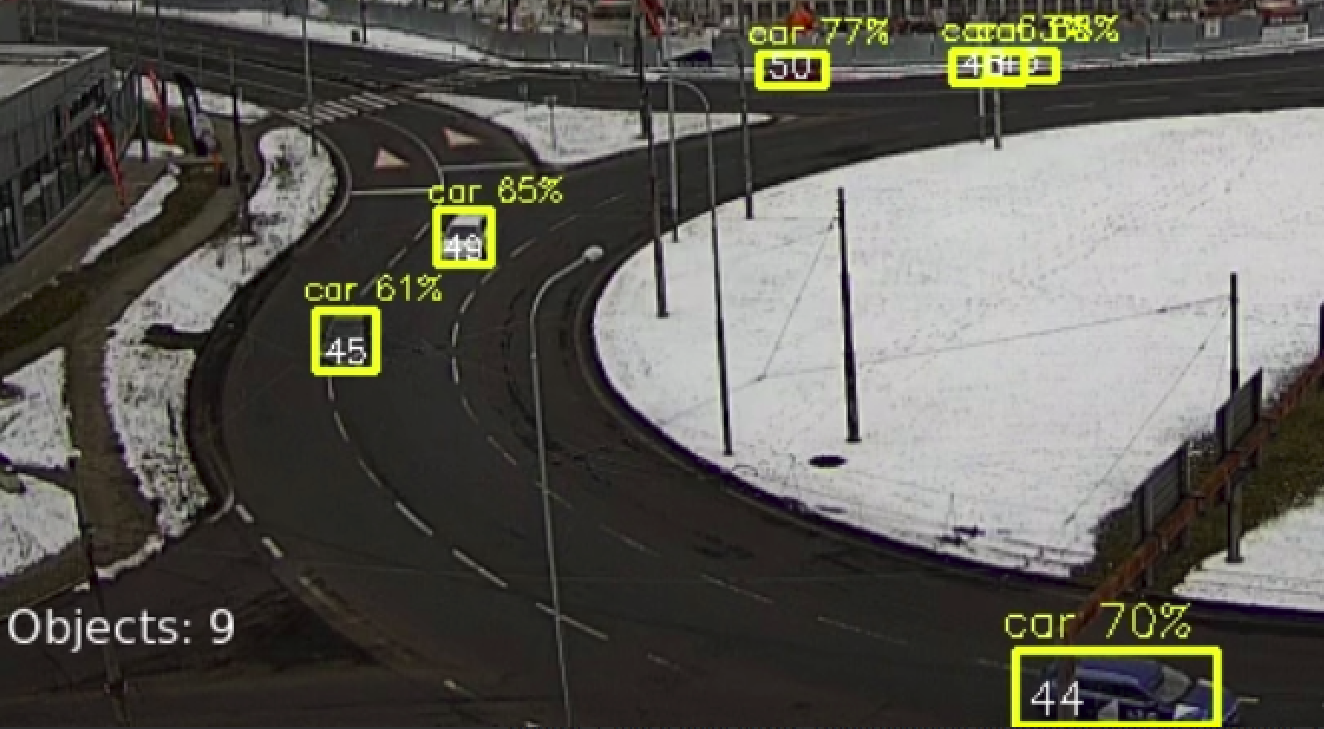
\includegraphics[width=0.9\textwidth]{images/own_tracking.png}
    \caption{Ukázka víceobjektového sledování vozidel s~přiřazenými časově konzistentními identifikátory (vlastní zpracování, akcelerátor Hailo-8)}
    \label{fig:own_tracking}
\end{figure}

Jak je znázorněno na obrázku~\ref{fig:own_tracking}, implementovaný systém umožňuje stabilní sledování většího množství objektů v~reálném čase, přičemž každému vozidlu zůstává zachováno jeho unikátní číslo i při pohybu napříč snímanou scénou.

\subsection{Algoritmy pro sledování objektů}
Mezi nejpoužívanější a nejefektivnější přístupy pro sledování objektů v~reálném čase patří algoritmy SORT a DeepSORT. Tyto metody jsou oblíbené zejména pro svou nízkou výpočetní náročnost, vysokou propustnost a snadnou integraci s~moderními detekčními modely, jako je rodina modelů \acs{YOLO}~\cite{redmon_yolo_2016}.


\subsubsection{SORT}
Algoritmus \acs{SORT} (z~angl. \textit{Simple Online and Realtime Tracking}) je postaven na kombinaci dvou klíčových komponent: Kalmanova filtru\footnote{Kalmanův filtr je rekurzivní matematický algoritmus, který ze série nepřesných a zašuměných měření (v~tomto případě historických detekcí z~kamery) odhaduje aktuální a predikuje budoucí stav dynamického systému (například polohu, směr a rychlost jedoucího vozidla).} a Maďarského algoritmu pro datovou asociaci. Kalmanův filtr slouží k~predikci budoucí polohy objektu v~následujícím snímku na základě lineárního pohybového modelu. Stav každého sledovaného objektu je definován vektorově pomocí souřadnic středu ohraničujícího obdélníku, jeho plochy (měřítka), poměru stran a jejich příslušných rychlostí změn v~čase.

Jakmile jsou v~novém snímku získány čerstvé detekce, nastupuje Maďarský algoritmus, který řeší optimalizační úlohu přiřazení predikovaných poloh k~reálným novým detekcím. Jako nákladová funkce (metrika vzdálenosti) se zde využívá překryv ohraničujících obdélníků vyjádřený pomocí metriky (\acs{IoU}, z~angl. \textit{Intersection over Union}). Díky této matematické přímočarosti dosahuje SORT extrémní rychlosti zpracování, avšak jeho zásadní nevýhodou je nestabilita při dlouhodobějších překryvech (okluzích) objektů, kdy absence vizuální informace často vede ke ztrátě stopy a fatálnímu selhání přiřazení \acs{ID}~\cite{SORT_original_2016}.

\begin{figure}[H]
    \centering
    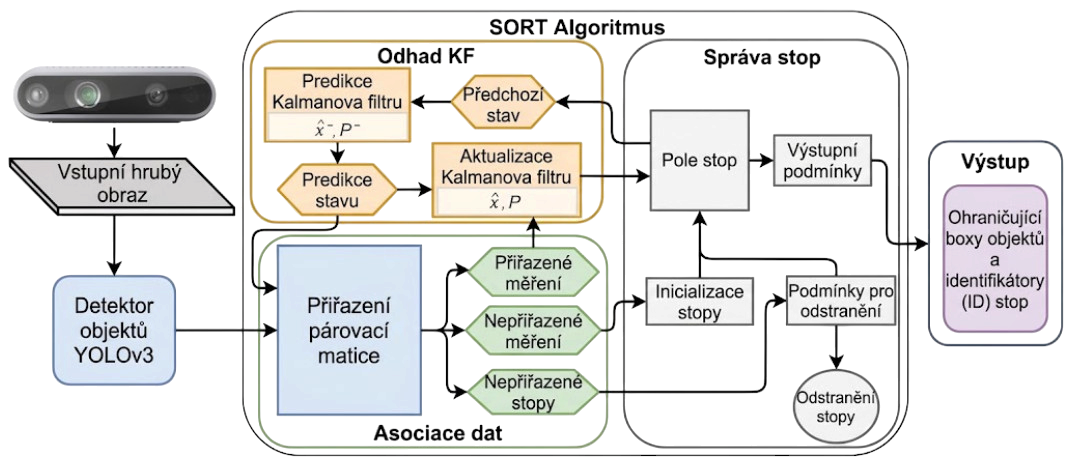
\includegraphics[width=1\textwidth]{images/sort_algorithm_principe_CZ.png}
    \caption{Celkový přehled a princip fungování sledovacího algoritmu \acs{SORT} (vlastní překlad, adaptováno z~\cite[s.~5]{pereira2022sort}).}
    \label{fig:sort_overview}
\end{figure}

%\begin{enumerate}
%    \item \textbf{Odhad Kalmanovým filtrem (z angl. \textit{KF Estimation}):} Tato část schématu představuje paměť systému. Na základě předchozího stavu (\textit{Previous State}) algoritmus provede matematickou predikci (\textit{Kalman Filter Prediction}), čímž získá odhadovanou polohu sledovaných objektů v aktuálním čase (\textit{State Prediction}).
%    \item \textbf{Asociace dat (z angl. \textit{Data Association}):} Do tohoto bloku vstupují jak odhadnuté polohy z Kalmanova filtru, tak zcela nové detekce z modelu YOLO. Úkolem párovací matice (\textit{Cost Matrix Matching}) je optimálně spojit tyto dva vstupy pomocí metriky \acs{IoU}. Výstupem jsou tři možné stavy: úspěšně spárovaná měření (\textit{Matched Measurement}), nové detekce bez historie (\textit{Unmatched Measurement}) a existující stopy, ke kterým se nenašla nová detekce (\textit{Unmatched Tracks}).
%    \item \textbf{Správa stop (z angl. \textit{Track Management}):} V závěrečné fázi systém reaguje na výsledky předchozí asociace. Spárovaná měření aktualizují Kalmanův filtr a udržují se v poli aktivních stop (\textit{Array of Tracks}). Z nespárovaných měření, což typicky představuje nově příchozí vozidla, se inicializují stopy nové (\textit{Track Initialization}). Nespárované stopy, tedy vozidla, která pravděpodobně opustila scénu, jsou po splnění stanovených podmínek ze systému odstraněny (\textit{Track Delete}). Validní stopy jsou následně propuštěny na finální výstup (\textit{Output}).
%\end{enumerate}

Na obrázku~\ref{fig:sort_overview} je detailně znázorněna celá pracovní smyčka (z~angl. \textit{pipeline}) algoritmu SORT~\cite{SORT_original_2016}, která se nezávisle opakuje s~každým novým obrazovým snímkem. Podle blokového schématu lze celý proces logicky rozdělit do tří na sebe navazujících fází:

\begin{enumerate}
    \item \textbf{Odhad KF:} Tato část schématu představuje paměť systému. Na základě předchozího stavu (\textit{Předchozí stav}) algoritmus provede matematickou predikci (\textit{Predikce Kalmanova filtru}), čímž získá odhadovanou polohu sledovaných objektů v~aktuálním čase (\textit{Predikce stavu}).
    \item \textbf{Asociace dat:} Do tohoto bloku vstupují jak odhadnuté polohy z~Kalmanova filtru, tak zcela nové detekce z~modelu YOLO. Úkolem párovací matice (\textit{Přiřazení párovací matice}) je optimálně spojit tyto dva vstupy pomocí metriky \acs{IoU}. Výstupem jsou tři možné stavy: úspěšně spárovaná měření (\textit{Přiřazené měření}), nové detekce bez historie (\textit{Nepřiřazené měření}) a existující stopy, ke kterým se nenašla nová detekce (\textit{Nepřiřazené stopy}).
    \item \textbf{Správa stop:} V~závěrečné fázi systém reaguje na výsledky předchozí asociace. Spárovaná měření aktualizují Kalmanův filtr a udržují se v~poli aktivních stop (\textit{Pole stop}). Z~nespárovaných měření, což typicky představuje nově příchozí vozidla, se inicializují stopy nové (\textit{Inicializace stopy}). Nespárované stopy, tedy vozidla, která pravděpodobně opustila scénu, jsou po splnění stanovených podmínek ze systému odstraněny (\textit{Odstranění stopy}). Validní stopy jsou následně propuštěny na finální výstup (\textit{Výstup}).
\end{enumerate}

\subsubsection{DeepSORT}
Algoritmus \acs{DeepSORT} (z~angl. \textit{Deep Simple Online and Realtime Tracking}) vznikl jako přímá reakce na slabá místa původního algoritmu SORT v~komplexních a hustých scénách. Rozšiřuje čistě geometrické a prostorové přiřazování o~integraci hlubokých konvolučních neuronových sítí, které jsou vytrénovány pro extrakci vizuálních vzhledových příznaků (z~angl. \textit{deep appearance descriptors}). Pro každý detekovaný objekt je vygenerován charakteristický vektor (embedding), který reprezentuje jeho vizuální identitu.

Při samotné asociaci dat pak DeepSORT kombinuje dvě metriky: Mahalanobisovu vzdálenost, která reflektuje pohybovou konzistenci na základě Kalmanova filtru, a kosinovou vzdálenost, jež vyhodnocuje shodu vizuálních příznaků s~historií daného objektu. Propojení těchto informací probíhá pomocí kaskádového párování (\textit{matching cascade}). Tento kombinovaný přístup dramaticky zvyšuje robustnost sledování v~hustém dopravním provozu, kde dochází k~častému vzájemnému zakrývání vozidel, a prokazatelně minimalizuje množství chyb typu záměny identity (\textit{\acs{ID} switches})~\cite{wojke_deepsort_2017}.

\begin{figure}[H]
    \centering
    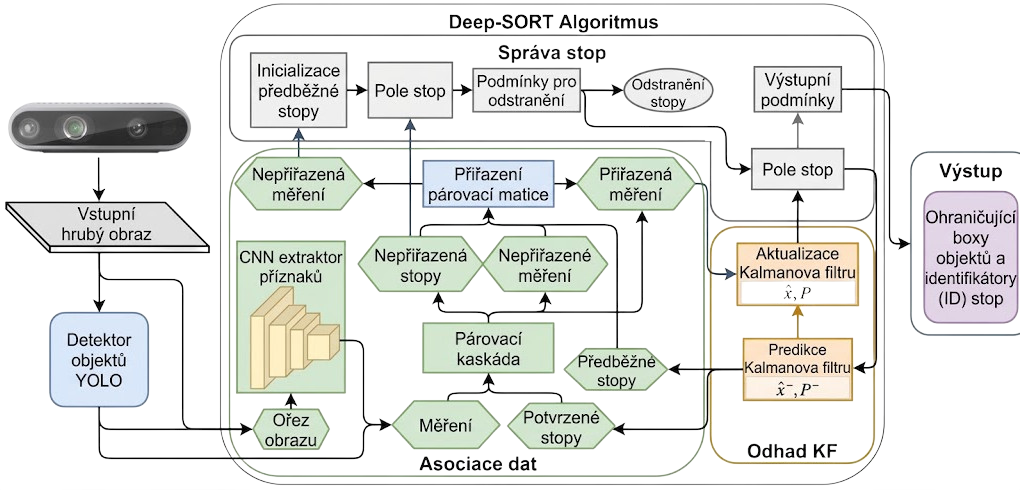
\includegraphics[width=1\textwidth]{images/deepsort_algorithm_principe_CZ.png}
    \caption{Blokové schéma architektury sledovacího algoritmu DeepSORT a jeho rozhodovacích kroků (vlastní překlad, adaptováno z ~\cite[s.~7]{pereira2022sort})}
    \label{fig:deepsort_overview}
\end{figure}

Na obrázku~\ref{fig:deepsort_overview} je detailně znázorněna architektura a datový tok algoritmu Deep-SORT. Podle blokového schématu lze celý proces rozdělit do následujících klíčových fází, které se vykonávají s~každým novým snímkem:

\begin{enumerate}
    \item \textbf{Extrakce příznaků a predikce polohy:} Vstupní obraz (\textit{Vstupní hrubý obraz}) je nejprve zpracován detektorem objektů, ze kterého jsou získány obrazové výřezy jednotlivých vozidel (\textit{Ořez obrazu}). Tyto výřezy následně zpracovává konvoluční neuronová síť (\textit{CNN extraktor příznaků}), jež extrahuje unikátní vizuální příznaky. Souběžně s~tím modul odhadu (\textit{Odhad KF}) provádí matematickou predikci budoucí polohy pomocí Kalmanova filtru (\textit{Predikce Kalmanova filtru}).
    
    \item \textbf{Asociace dat:} Tento centrální modul kombinuje nová měření obohacená o~vizuální příznaky (\textit{Měření}) a potvrzené stopy z~minulosti (\textit{Potvrzené stopy}). Klíčovým inovačním prvkem oproti původnímu algoritmu SORT je kaskádové párování (\textit{Párovací kaskáda}), které prioritně využívá právě vizuální podobnost. Objekty a měření, které kaskáda nedokáže spojit (\textit{Nepřiřazené stopy} a \textit{Nepřiřazená měření}), jsou zachyceny a předány do klasické párovací matice (\textit{Přiřazení párovací matice}), jež funguje jako záloha využívající standardní prostorový překryv.
    
    \item \textbf{Správa stop a aktualizace:} Výstupy z~asociace dat se dělí do tří směrů. Úspěšně spárovaná měření (\textit{Přiřazená měření}) jsou využita k~okamžité aktualizaci Kalmanova filtru (\textit{Aktualizace Kalmanova filtru}). Zcela nová detekovaná vozidla, která nemají historii (\textit{Nepřiřazená měření}), zakládají v~systému nové, zatím nepotvrzené stopy (\textit{Inicializace předběžné stopy}). Správa stop následně kontroluje celé pole aktivních záznamů (\textit{Pole stop}). Vozidla, jež dlouhodobě chybí a splní podmínky pro smazání (\textit{Podmínky pro odstranění}), jsou ze systému odstraněna (\textit{Odstranění stopy}). Stopy splňující výstupní kritéria (\textit{Výstupní podmínky}) jsou předány na finální výstup v~podobě souřadnic a unikátních identifikátorů (\textit{Výstup}).
\end{enumerate}

\subsection{Metody sčítání objektů}
Samotné automatické sčítání objektů v~dopravním proudu bezprostředně navazuje na výsledky získané z~MOT. Namísto prosté kumulace detekcí v~jednotlivých samostatných snímcích, která by vedla k~masivnímu nadhodnocení výsledků (například z~důvodu vícenásobného započítání téhož stojícího či pomalu jedoucího vozidla), se využívá analýzy časoprostorových trajektorií jednoznačně identifikovaných objektů~\cite{zhou_traffic_survey_2024}.

V~praxi se pro automatizované sčítání a kategorizaci využívají dva primární koncepční přístupy:
\begin{itemize}
    \item \textbf{Virtuální čára (z~angl. \textit{Virtual Line}):} Jedná se o~nejrozšířenější a výpočetně nejméně náročnou metodu pro sčítání vozidel v~konkrétních jízdních pruzích či směrech. V~obrazovém prostoru je definována úsečka fungující jako detekční brána. Systém v~každém kroku kontroluje, zda vektor trajektorie konkrétního objektu (typicky reprezentovaný středovým nebo spodním bodem jeho ohraničujícího obdélníku) protnul tuto linii. V~okamžiku detekce průsečíku je inkrementováno počítadlo pro daný směr jízdy. Tento přístup je vysoce efektivní pro stanovení okamžité intenzity dopravy na liniových úsecích komunikací~\cite{zhou_traffic_survey_2024}.
    \item \textbf{Oblast zájmu (\acs{ROI}, z~angl. \textit{Region of Interest}):} Alternativní přístup spočívá ve vymezení uzavřené polygonální nebo obdélníkové zóny přímo v~digitálním obraze. Sledovaný objekt je zaregistrován a statisticky započítán buď v~momentě vstupu do této definované oblasti, nebo při jejím opuštění. Tento princip se využívá především v~situacích, kde je nutné sledovat celkovou obsazenost určitého vyhrazeného prostoru (např. plochy křižovatek, odbočovací pruhy nebo parkoviště) či analyzovat průměrnou dobu zdržení vozidel v~daném segmentu~\cite{szeliski_computer_vision, zhou_traffic_survey_2024}.
\end{itemize}

\begin{figure}[H]
    \centering
    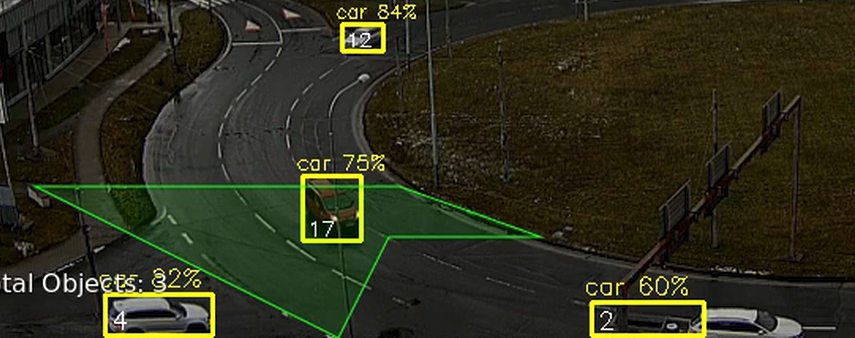
\includegraphics[width=1\textwidth]{images/own_objects_tracking.png}
    \caption{Definice analytické oblasti zájmu (\acs{ROI}) pomocí polygonu v~praktické implementaci sledovacího systému (vlastní zpracování, akcelerátor Hailo-8).}
    \label{fig:own_roi_polygon}
\end{figure}

Jak ukazuje obrázek~\ref{fig:own_roi_polygon}, zatímco na rovných úsecích komunikací často postačuje k~detekci průjezdu jednoduchá virtuální čára, složitější dopravní uzly, jakými jsou kruhové objezdy, vyžadují robustnější přístup. V~rámci předložené implementace je proto oblast zájmu (\acs{ROI}) definována jako nepravidelný n-úhelník (polygon). Tento geometrický útvar je v~systému konstruován pomocí přesné sady 2D souřadnic (vrcholů) definovaných v~obrazovém prostoru předzpracovaného snímku.

Proces samotného sčítání a vyhodnocování trajektorií je následně založen na průběžném výpočtu prostorového průniku (z~angl. \textit{spatial intersection}). Systém v~každém snímku kontinuálně extrahuje polohu sledovaných objektů, jež jsou typicky reprezentovány středovým bodem (centroidem) jejich ohraničujícího obdélníku. Jakmile vyhodnocovací algoritmus detekuje, že se tento referenční bod vozidla nachází přímo uvnitř definované polygonové zóny (což matematicky odpovídá úloze bodu v~polygonu, tzv. \textit{Point-in-Polygon}), je vozidlo okamžitě započítáno do celkové statistiky dopravy. Tento moment je na obrázku názorně zachycen u~objektu s~identifikátorem 17. Tento plošný přístup výrazně eliminuje chyby spojené s~nepřesnostmi detekce na hranách a umožňuje spolehlivé sčítání i při zakřivených a překrývajících se trajektoriích.


\section{Počítačové vidění pro analýzu dopravy}
Počítačové vidění (z~angl. \textit{Computer Vision}) představuje interdisciplinární oblast informatiky, která se zabývá automatickou analýzou statických snímků a videozáznamů. Jeho hlavním cílem je extrakce relevantních a sémantických informací z~vizuálních vstupů. V~oblasti moderních dopravních systémů je počítačové vidění využíváno zejména v~aplikacích dopravního dohledu, proaktivního řízení provozu a při automatické analýze dopravní propustnosti. Kamerové systémy umožňují kontinuální sledování dopravních toků, detekci anomálních situací nebo identifikaci konkrétních vozidel a jejich registračních značek~\cite{szeliski_computer_vision, zhou_traffic_survey_2024}.

\subsection{Předzpracování obrazu}
Předzpracování obrazu představuje nezbytný přípravný krok před samotnou aplikací detekčních modelů. Cílem je zlepšení kvality vstupních dat, potlačení digitálního šumu a optimalizace celkové výpočetní zátěže. 

V~dopravních aplikacích je surový videozáznam z~kamery často výpočetně příliš objemný a obsahuje velké množství irelevantních informací (např. oblohu, okolní budovy, chodníky). Prvním logickým krokem je proto definice oblasti zájmu (\acs{ROI}). Softwarové oříznutí nebo zavedení masky zaručí, že systém analyzuje pouze samotnou vozovku. To nejen radikálně snižuje objem zpracovávaných dat, ale také eliminuje falešné detekce, jako jsou například zaparkovaná vozidla mimo zorné pole křižovatky.

Následně musí být upravený obraz transformován do formátu, který striktně vyžaduje architektura neuronové sítě. Jedná se primárně o~\textbf{škálování (z~angl. \textit{resizing})} na fixní rozlišení (typicky $640 \times 640$). Aby při změně velikosti nedošlo k~deformaci poměru stran, což by zhoršilo schopnost sítě rozeznat tvar a proporce vozidla, využívá se běžně technika zvaná \textit{letterboxing}. Ta zmenší obraz proporcionálně a chybějící prostor (okraje) doplní neutrální barvou. 

Poslední rutinní fází je \textbf{normalizace barev}. Hodnoty jednotlivých pixelů, které standardně nabývají celočíselných hodnot 0 až 255, jsou převedeny na desetinná čísla v~intervalu 0,0 až 1,0. Tento krok stabilizuje a výrazně urychluje matematické výpočty (násobení matic) uvnitř umělé neuronové sítě~\cite{szeliski_computer_vision}. I~přes tuto důkladnou datovou optimalizaci však analýza obrazu zůstává nesmírně výpočetně náročná, což představuje hlavní výzvu při nasazení na okrajových zařízeních.

\begin{figure}[H]
    \centering
    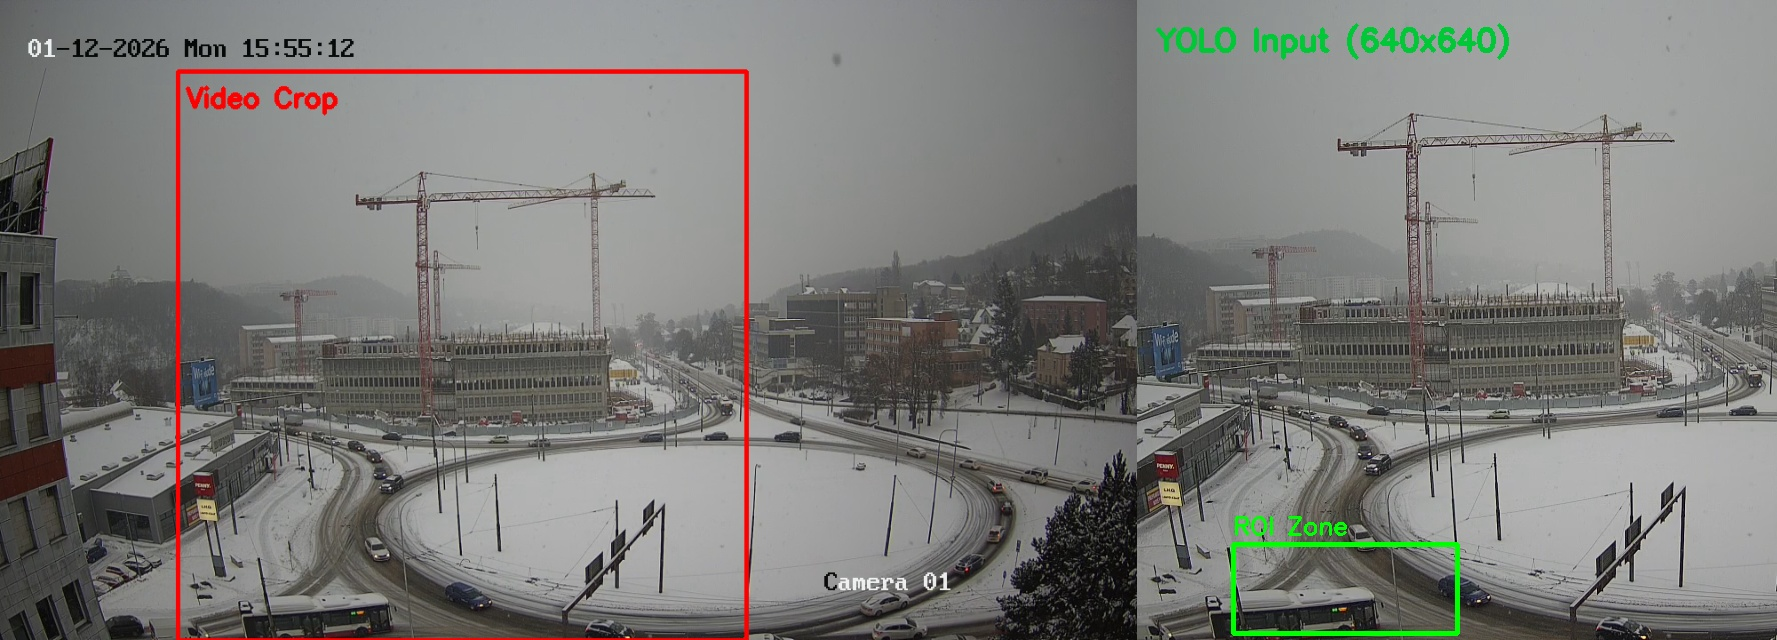
\includegraphics[width=\textwidth]{images/preprocessing_gstreamer.jpg}
    \caption{Příklad dvoufázového vymezení oblasti zájmu, hardwarový ořez vlevo a softwarová analytická zóna vpravo (vlastní zpracování).}
    \label{fig:image_preprocessing}
\end{figure}

Jak ukazuje obrázek~\ref{fig:image_preprocessing}, předzpracování obrazového toku hraje klíčovou roli v~optimalizaci celého systému. Namísto výpočetně náročnějších metod (jako je doplňování černých pruhů u~\textit{letterboxingu}) je v~navrženém systému využit přímý prostorový ořez obrazu (z~angl. \textit{crop}). Levá část obrázku znázorňuje zdrojový snímek, který byl v~rámci datovodu nejprve naškálován na rozlišení $1280\times720$ pixelů. Červený obdélník v~něm přesně vymezuje hranice hardwarového ořezu ten je definován počátečními souřadnicemi $x=200, y=80$ s~pevnou šířkou a výškou $640$ pixelů. 

Pravá část následně představuje fyzicky vyříznutý čtverec, jenž svými rozměry ($640\times640$) nativně odpovídá požadavkům vstupní vrstvy modelu YOLO. Je nutné zdůraznit, že tento hardwarový ořez slouží výhradně k~obrazové přípravě dat před vstupem do modelu. Samotná analytická oblast zájmu (\acs{ROI}), která určuje, kde reálně dochází k~detekci a sčítání vozidel, je v~systému definována až následně. Na pravé části obrázku je tato aplikační logika vizualizována zeleným obdélníkem. Jeho poloha je v~aplikačním kódu dynamicky vypočítávána pomocí relativních souřadnic vůči velikosti předzpracovaného výstupu (v~tomto konkrétním případě $x=96, y=544, w=224, h=90$). Oddělením těchto dvou fází je do neuronové sítě propuštěn čistší datový tok, přičemž analytika si zachovává plnou flexibilitu.

\subsection{Základní úlohy počítačového vidění}
V~rámci analýzy dopravy a návrhu inteligentní dopravní infrastruktury se počítačové vidění opírá o~tři základní, na sebe úzce navazující úlohy:

\begin{itemize}
    \item \textbf{Detekce objektů:} Zaměřuje se na samotnou lokalizaci objektů v~obraze. Výstupem této úlohy jsou obvykle ohraničující obdélníky (z~angl. \textit{bounding boxes}), které vymezují prostorovou polohu nalezených entit. V~dopravních aplikacích se jedná především o~detekci vozidel, chodců nebo cyklistů.
    \item \textbf{Klasifikace objektů:} Představuje úlohu, při které je již detekovanému objektu přiřazena předem definovaná třída na základě jeho vizuálních charakteristik. V~praxi se využívá například pro rozlišení, zda je detekované vozidlo osobní automobil, nákladní vůz nebo autobus~\cite{szeliski_computer_vision}.
    \item \textbf{Sledování objektů:} Umožňuje analyzovat pohyb detekovaných a klasifikovaných objektů napříč po sobě jdoucími snímky video sekvence. Slouží k~odhadu trajektorií, predikci směru a výpočtu rychlosti pohybu~\cite{zhou_traffic_survey_2024}.
\end{itemize}

\begin{figure}[H]
    \centering
    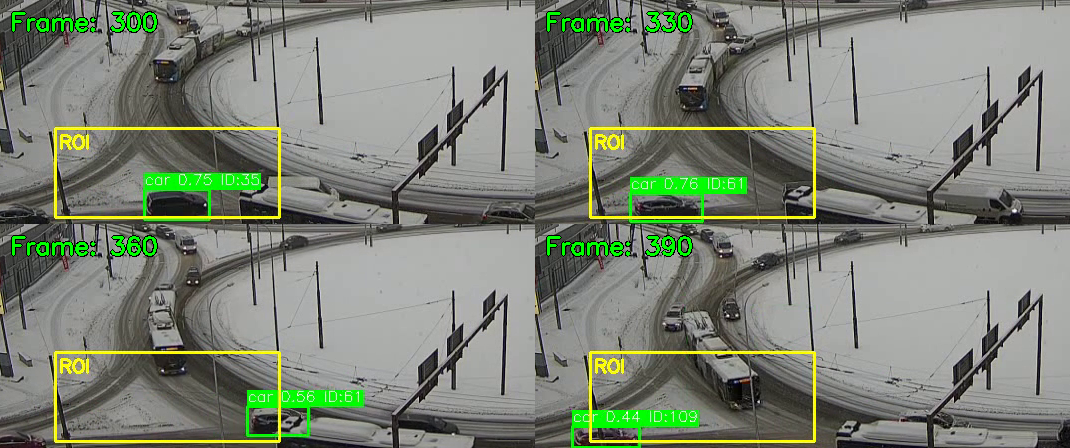
\includegraphics[width=1\textwidth]{images/tracking_grid_final.png}
    \caption{Časová sekvence čtyř snímků demonstrující kontinuální sledování objektů a vyhodnocování jejich polohy vůči definované zóně (ROI). Systém úspěšně udržuje \acs{ID} u~projíždějícího automobilu a dynamicky registruje nová vozidla (vlastní zpracování, inference na GPU).}
    \label{fig:object_tracking_example}
\end{figure}

Jak je názorně ukázáno na obrázku~\ref{fig:object_tracking_example}, propojení úlohy detekce a sledování umožňuje systému přidělit jednotlivým vozidlům unikátní identifikátory (\acs{ID}) a kontinuálně je sledovat v~čase. Obrázek zachycuje sekvenci čtyř po sobě jdoucích snímků s~pevným rozestupem 30 rámečků (snímky 300, 330, 360 a 390). Vzhledem k~tomu, že zdrojové video je zpracováváno frekvencí 15 snímků za sekundu (FPS), představuje časový krok mezi každým zobrazeným dílčím obrázkem přesně 2 sekundy reálného času (celá mřížka tak mapuje celkem 6 sekund dopravního provozu). Pro každé detekované vozidlo systém neustále vypočítává středový bod (centroid) jeho ohraničujícího obdélníku. Zásadní analytickou podmínkou je, že vozidlo je do statistik průjezdů aktivně zahrnuto pouze tehdy, nachází-li se tento vypočítaný střed fyzicky uvnitř definované oblasti zájmu (žlutý obdélník \acs{ROI}).

Plynulý průjezd a spolehlivost sledování jsou prokazatelně demonstrovány na osobním automobilu (označeném jako \textit{car ID:61}). Toto vozidlo je zachyceno ve sledované zóně \acs{ROI} ve snímku 330, přičemž o~dvě sekundy později (snímek 360) si systém navzdory jeho pohybu napříč křižovatkou úspěšně udržuje jeho původní \acs{ID}. Z~mřížky je rovněž jasně patrné, jak algoritmus dynamicky reaguje na celkovou obměnu vozidel ve scéně. Zatímco na prvním snímku (300) zónou projíždí předchozí vozidlo s~\acs{ID} 35, na posledním snímku (390) do \acs{ROI} zleva vstupuje další automobil, kterému systém okamžitě a správně přiděluje nové, dosud nepoužité \acs{ID} (109). Tento holistický přístup, kombinující striktní prostorové omezení analytickou zónou a konzistentní sledování identity napříč snímky, je v~dopravních aplikacích naprosto klíčový pro zabránění falešnému vícenásobnému započítání téhož objektu.

\section{Přehled detekčních modelů}
V~posledních letech dominují oblasti detekce objektů architektury hlubokých konvolučních neuronových sítí (CNN). Pro nasazení na výpočetně omezených okrajových zařízeních se historicky osvědčily zejména modely z~rodiny SSD a YOLO, které patří do kategorie tzv. jednofázových detektorů (z~angl. \textit{one-stage detectors}). Tyto modely dokáží obraz zpracovat během jediného průchodu sítí, čímž splňují výše zmíněné požadavky na nízkou latenci.

Architektura \acs{SSD} (z~angl. \textit{Single Shot MultiBox Detector}) detekuje objekty tak, že využívá hustou sadu předem definovaných kotevních obdélníků (z~angl. \textit{anchor boxes}) o~různých poměrech stran a velikostech. Predikce probíhá na několika mapách příznaků s~různým rozlišením současně, což modelu teoreticky umožňuje lépe zachytit objekty nejrůznějších velikostí~\cite{szeliski_computer_vision}.

%Ačkoliv \ac{SSD} dosahuje stabilní přesnosti, v kontextu nasazení na vysoce omezeném hardwaru nedosahuje takové efektivity jako inovativnější přístupy. Z tohoto důvodu byl pro praktickou implementaci v této bakalářské práci zvolen model z rodiny YOLO. Tento model nabízí bezkonkurenční poměr mezi přesností detekce a propustností snímků a disponuje vynikající softwarovou podporou pro následnou kompilaci a optimalizaci na dedikovaných AI akcelerátorech.

\subsection{Model YOLO}
Ačkoliv SSD dosahuje stabilní přesnosti, naprostou revoluci v~efektivitě přinesla architektura \acs{YOLO} (z~angl. \textit{You Only Look Once}), která od základů transformovala přístup k~počítačovému vidění. Namísto dvoufázového generování návrhů oblastí (jako u~starších sítí \acs{R-CNN}, z~angl. \textit{Region-based Convolutional Neural Network}) formuluje detekci jako jedinou, \textit{end-to-end} regresní úlohu~\cite{redmon_yolo_2016}.

\begin{figure}[H]
    \centering    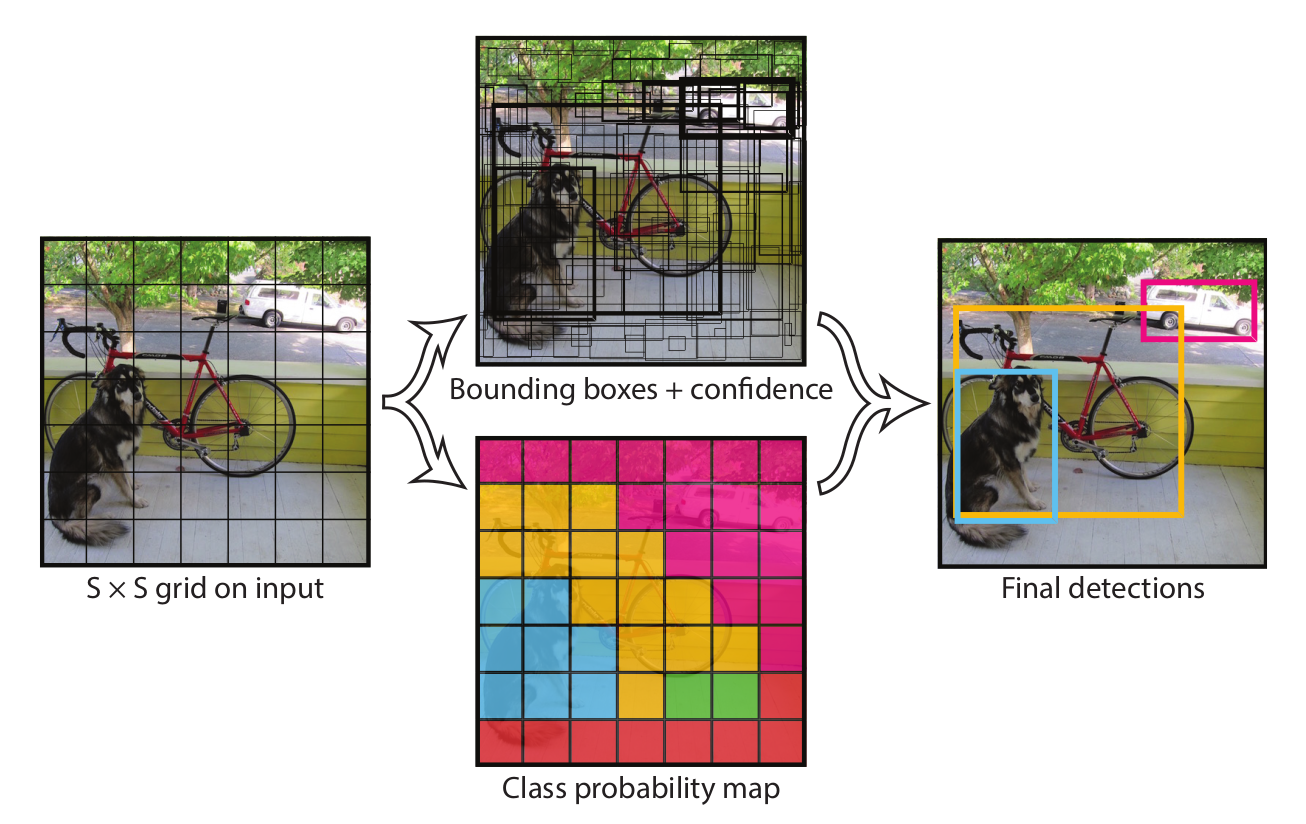
\includegraphics[width=1\textwidth]{images/yolo_v1_diagram.png}
    \caption{Základní princip detekce modelu YOLO využívající rozdělení obrazu do mřížky (převzato z~\cite[s.~2]{redmon_yolo_2016})}
    \label{fig:detection_principe}
\end{figure}

Jak ukazuje obrázek~\ref{fig:detection_principe}, vstupní obraz je nejprve virtuálně rozdělen do mřížky $S \times S$. Pokud střed hledaného objektu spadne geometricky do konkrétní buňky této mřížky, stává se tato konkrétní buňka plně zodpovědnou za jeho detekci. Každá buňka následně predikuje fixní počet $B$ ohraničujících obdélníků, míru spolehlivosti (z~angl. \textit{confidence score}) pro tyto obdélníky a pravděpodobnosti zařazení do $C$ různých tříd. Celkový výstup sítě je tak elegantně zakódován do jediného tenzoru o~rozměrech $S \times S~\times (B \cdot 5 + C)$.

\begin{figure}[H]
    \centering
    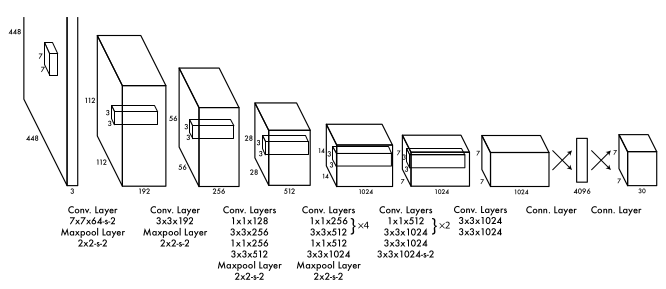
\includegraphics[width=1\textwidth]{images/yolo_model_conv.png}
    \caption{Vnitřní architektura modelu YOLO znázorňující sekvenci konvolučních a plně propojených vrstev (převzato z~\cite[s.~3]{redmon_yolo_2016})}
    \label{fig:yolo_arch}
\end{figure}
Na obrázku~\ref{fig:yolo_arch} je detailně znázorněna topologie vrstev původního modelu \acs{YOLO}, jejíž architektura byla přímo inspirována modelem GoogLeNet\footnote{GoogLeNet (známý také pod označením Inception v1) je průlomová architektura hluboké konvoluční neuronové sítě od společnosti Google, která v~roce 2014 zvítězila v~prestižní soutěži počítačového vidění ImageNet (ILSVRC). Vyznačuje se velmi vysokou výpočetní efektivitou.}. Systém na svém vstupu přijímá obraz o~přesném rozlišení $448 \times 448$ pixelů. Samotná síť se skládá z~24 konvolučních vrstev, které slouží k~postupné a hluboké extrakci vizuálních příznaků z~obrazu (od jednoduchých hran až po komplexní tvary vozidel). Za nimi následují 2 plně propojené vrstvy (z~angl. \textit{fully connected layers}), jež získané příznaky agregují a generují finální predikční tenzor o~rozměrech $7 \times 7 \times 30$.

Klíčovým inovačním prvkem této architektury je zařazení střídavých redukčních konvolučních vrstev s~filtrem $1 \times 1$. Tyto vrstvy fungují jako informační úzká hrdla (z~angl. \textit{bottlenecks}) – efektivně zmenšují prostor příznaků z~předchozích vrstev, čímž drasticky redukují množství potřebných matematických operací bez zásadní ztráty kontextu. Moderní varianty modelů z~rodiny YOLO jsou pro účely přesné objektové detekce standardně trénovány a vyhodnocovány na rozsáhlém datasetu COCO\footnote{\href{https://www.kaggle.com/datasets/erennik/coconames}{COCO dataset}} (z~angl. \textit{Common Objects in Context})~\cite{lin_coco_2014}. Tento dataset obsahuje stovky tisíc detailně anotovaných snímků reálných scén a plně definuje 80 základních tříd objektů, což detekčnímu modelu poskytuje vysoce robustní výchozí základ pro spolehlivé rozpoznávání různorodých účastníků dopravního provozu (osobní automobily, autobusy, nákladní vozy či chodce).

\subsection{Architektura a škálování variant modelu YOLOv8}
Významný architektonický posun přinesla generace modelů \textbf{YOLOv8}, vyvinutá společností Ultralytics~\cite{terven_yolo_review_2023, jocher_yolov8_2023}. Oproti starším generacím opouští YOLOv8 koncept předdefinovaných kotevních obdélníků a zavádí plně bezkotevní (\textit{anchor-free}) detekci, která přímo predikuje střed objektu a jeho vzdálenosti k~hranám ohraničujícího rámečku. Detekční hlava je navíc rozdělena (\textit{decoupled head}) na dvě nezávislé větve – jedna řeší výhradně klasifikaci tříd pomocí binární křížové entropie (BCE) a druhá prostorovou regresi souřadnic pomocí ztrátových funkcí CIoU a DFL (\textit{Distribution Focal Loss}). V~páteřní síti (\textit{backbone}) a krku (\textit{neck}) byl starší konvoluční blok C3 nahrazen novým stavebním modulem \textbf{C2f} (\textit{CSP Bottleneck with 2 convolutions}), který propojuje příznaky z~více mezivrstev a zajišťuje bohatší tok gradientů při zachování nízké výpočetní náročnosti~\cite{terven_yolo_review_2023}.

Aby bylo možné tutéž architekturu nasadit jak na extrémně úsporných mikropočítačích, tak na výkonných cloudových serverech, je rodina YOLOv8 rozdělena do pěti velikostních variant: \textbf{Nano (\texttt{n})}, \textbf{Small (\texttt{s})}, \textbf{Medium (\texttt{m})}, \textbf{Large (\texttt{l})} a \textbf{Extra Large (\texttt{x})}~\cite{jocher_yolov8_2023}. Všechny tyto varianty sdílejí totožnou makro-architekturu (stejné pořadí konvolučních vrstev, bloků C2f a vrstvy SPPF), ale liší se hodnotou tří škálovacích koeficientů (\textit{compound scaling constants})~\cite{terven_yolo_review_2023, jocher_yolov8_2023}:
\begin{itemize}
    \item \textbf{Hloubkový multiplikátor ($d$, \texttt{depth\_multiple}):} Určuje, kolikrát se uvnitř každého modulu C2f opakují vnitřní reziduální bloky (\textit{Bottleneck}). Tím přímo řídí celkový počet vrstev neuronové sítě – menší modely \texttt{YOLOv8n} a \texttt{YOLOv8s} ($d=0{,}33$) čítají v~neslitém výpočetním grafu \textbf{225 vrstev} (168 vrstev po fúzi konvoluce a dávkové normalizace při inferenci), střední model \texttt{YOLOv8m} ($d=0{,}67$) obsahuje \textbf{295 vrstev} (218 po fúzi) a největší modely \texttt{YOLOv8l} a \texttt{YOLOv8x} ($d=1{,}00$) dosahují hloubky \textbf{365 vrstev} (268 po fúzi).
    \item \textbf{Šířkový multiplikátor ($w$, \texttt{width\_multiple}):} Škáluje počet konvolučních filtrů (výstupních kanálů) v~každé vrstvě sítě v~rozsahu od $w=0{,}25$ (varianta \texttt{n}) až po $w=1{,}25$ (varianta \texttt{x}). Růst šířky sítě kvadraticky zvyšuje počet trénovatelných parametrů i nároky na výpočetní výkon (GFLOPs).
    \item \textbf{Maximální počet kanálů ($c_{\max}$, \texttt{max\_channels}):} Omezuje horní hranici počtu kanálů v~nejhlubších vrstvách sítě (1\,024 kanálů pro \texttt{n}/\texttt{s}, 768 pro \texttt{m} a 512 pro \texttt{l}/\texttt{x}), aby u~hlubokých modelů nedocházelo k~neúměrnému nárůstu paměťové stopy.
\end{itemize}

Srovnání všech pěti variant při vstupním rozlišení $640 \times 640$~pixelů na referenčním datasetu \acs{COCO} val2017 shrnuje tabulka~\ref{tab:yolov8_variants}.

\begin{table}[H]
    \centering
    \small\renewcommand{\arraystretch}{1.2}
    \setlength{\tabcolsep}{3pt}
    \begin{tabular}{|l|c|c|c|c|c|c|}
        \hline
        \textbf{Varianta} & \textbf{Hloubka ($d$)} & \textbf{Šířka ($w$)} & \textbf{Počet vrstev (fúze)} & \textbf{Parametry} & \textbf{Výpočty (FLOPs)} & \textbf{$\text{mAP}_{50-95}$} \\ \hline
        \textbf{YOLOv8n} & 0,33 & 0,25 & 225 (168) & 3,2~M & 8,7~GFLOPs & 37,3~\% \\ \hline
        \textbf{YOLOv8s} & 0,33 & 0,50 & 225 (168) & 11,2~M & 28,6~GFLOPs & 44,9~\% \\ \hline
        \textbf{YOLOv8m} & 0,67 & 0,75 & 295 (218) & 25,9~M & 78,9~GFLOPs & 50,2~\% \\ \hline
        \textbf{YOLOv8l} & 1,00 & 1,00 & 365 (268) & 43,7~M & 165,2~GFLOPs & 52,9~\% \\ \hline
        \textbf{YOLOv8x} & 1,00 & 1,25 & 365 (268) & 68,2~M & 257,8~GFLOPs & 53,9~\% \\ \hline
    \end{tabular}
    \caption{Teoretické porovnání architektury a parametrů variant modelu YOLOv8 při vstupním rozlišení $640 \times 640$~px na datasetu COCO val2017~\cite{terven_yolo_review_2023, jocher_yolov8_2023}.}
    \label{tab:yolov8_variants}
\end{table}

Jak vyplývá z~tabulky~\ref{tab:yolov8_variants}, přechod od nejmenší varianty \texttt{YOLOv8n} ke střední variantě \textbf{\texttt{YOLOv8m}} (zvolené pro implementaci na akcelerátoru Hailo-8 v~této práci) přináší skokové zvýšení detekční přesnosti $\text{mAP}_{50-95}$ z~37,3~\% na 50,2~\% díky hlubší extrakci příznaků v~295 vrstvách. Naopak další zvětšování modelu na varianty \texttt{l} a \texttt{x} již přináší pouze mírný nárůst přesnosti (o~2,7 až 3,7 procentního bodu), avšak za cenu dvojnásobného až trojnásobného nárůstu výpočetní složitosti (GFLOPs), což je pro okrajová zařízení s~omezenou pamětí neefektivní.

\section{Systémy pro monitorování dopravy}
Monitorování dopravy představuje klíčovou součást moderních inteligentních dopravních systémů. Jeho primárním cílem je kontinuální získávání informací o~dopravním provozu, jako je intenzita dopravy, průměrná rychlost vozidel, detekce kongescí nebo výskyt nestandardních dopravních událostí. Tyto agregované informace jsou následně využívány pro aktivní řízení dopravy, strategické plánování městské infrastruktury a zvyšování celkové bezpečnosti silničního provozu~\cite{zhou_traffic_survey_2024}.

\subsection{Tradiční metody dopravního monitoringu}
Tradiční metody monitorování dopravy jsou historicky založeny převážně na fyzických kontaktních senzorech nebo manuálním sběru dat. Mezi jejich hlavní výhody patří relativně přímočará implementace a dlouhodobé ověření v~praxi, zásadní nevýhodou je však jejich omezená flexibilita, neschopnost poskytovat hlubší kontext a vysoké náklady na instalaci i následnou údržbu.

Jednou z~nejstarších metod je manuální sčítání dopravy, při kterém jsou dopravní prostředky zaznamenávány lidským pozorovatelem. Tento přístup je extrémně časově i personálně náročný, náchylný k~lidským chybám způsobeným únavou a je naprosto nevhodný pro kontinuální dlouhodobý monitoring dopravního provozu~\cite{zhou_traffic_survey_2024}.

Další široce rozšířenou technologií jsou indukční smyčky zabudované přímo do povrchu vozovky, které detekují přítomnost kovového podvozku vozidla na základě změny elektromagnetického pole. Ačkoliv poskytují relativně spolehlivá data o~prostých průjezdech vozidel, jejich instalace vyžaduje destruktivní zásah do vozovky, což omezuje dopravu. Samotné smyčky navíc podléhají rychlému opotřebení vlivem zátěže a povětrnostních podmínek~\cite{zhou_traffic_survey_2024}.

Pro monitorování rychlosti a vzdálenosti jsou rovněž hojně využívány radarové a lidarové senzory. Tyto technologie dosahují vysoké přesnosti i za zhoršené viditelnosti, avšak jejich nevýhodou jsou vysoké pořizovací náklady a omezené možnosti vizuální klasifikace jednotlivých typů objektů (např. obtížné rozlišení mezi malým motocyklem a chodcem)~\cite{zhou_traffic_survey_2024}.

% pridat obrazek tuzka papir, mobil s kategoriema
\subsection{Moderní kamerové systémy}
S~raketovým rozvojem počítačového vidění a dostupností vysokého výpočetního výkonu se v~dopravní infrastruktuře stále častěji prosazují kamerové systémy založené na analýze obrazových dat. Na rozdíl od jednorozměrných dat z~indukčních smyček umožňují kamerové systémy získávat z~jednoho zařízení bohaté, vícerozměrné informace o~celé dopravní scéně, včetně přesného typu vozidel, jejich trajektorií nebo anomálního chování účastníků provozu~\cite{szeliski_computer_vision}.

Mezi hlavní výhody těchto systémů patří vysoká flexibilita (změna sledované oblasti často vyžaduje pouze softwarovou úpravu virtuálních čar, nikoliv překopání vozovky) a možnost využití jedné kamery pro paralelní běh více analytických úloh. Nevýhodou kamerových systémů jsou naopak jejich limity spojené s~kvalitou vstupních obrazových dat. Výkon detekčních a sledovacích algoritmů může být negativně ovlivněn prudkými změnami světelných podmínek, nepříznivým počasím (mlha, hustý déšť) nebo vzájemným vizuálním překrýváním objektů ve scéně. Tyto faktory představují výzvu zejména v~hustém městském provozu~\cite{zhou_traffic_survey_2024}.

\subsubsection{Vstupní zařízení kamerových systémů}

\begin{figure}[H]
    \centering
    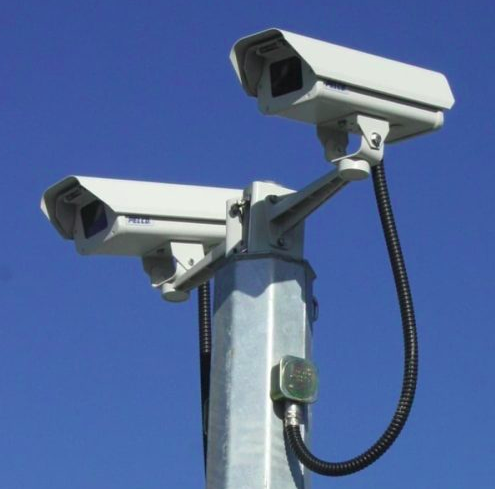
\includegraphics[width=0.5\textwidth]{images/traffic_camera.jpg}
    \caption{Typické umístění dohledových \acs{IP} kamer na sloupu infrastruktury. Toto neinvazivní řešení poskytuje stabilní obrazový tok pro následnou detekci a inferenci na okrajových zařízeních (převzato z~\cite{zdroj_kamera}).}
    \label{fig:traffic_camera}
\end{figure}

Pro zajištění kvalitního obrazového vstupu, který je pro algoritmy počítačového vidění kritický, se v~moderních systémech \acs{Edge AI} využívají primárně dva typy snímacích zařízení, jež přímo reflektují potřeby vývoje i reálného nasazení v~dopravní infrastruktuře:

\begin{itemize}
    \item \textbf{\acs{IP} kamery:} Představují současný standard v~budování chytrých měst. Tato zařízení nejenže snímají obraz, ale rovnou ho digitálně kódují a odesílají prostřednictvím počítačové sítě (nejčastěji pomocí protokolů \acs{RTSP} nebo \acs{ONVIF}). Jejich obrovskou výhodou je snadná integrace do existující síťové infrastruktury a možnost napájení přes jeden datový kabel (technologie \acs{PoE}). Pro účely detekce na okrajových zařízeních poskytují \acs{IP} kamery ideální a stabilní zdroj datového toku, ze kterého systém v~reálném čase extrahuje jednotlivé snímky pro inferenci.
    
    \item \textbf{Kamerové moduly s~přímým rozhraním (např. senzory Sony IMX):} Jedná se o~kompaktní kamerové moduly navržené pro přímé hardwarové připojení k~jednodeskovým počítačům (jako je platforma Raspberry Pi) pomocí vysokorychlostní sběrnice MIPI CSI. Zásadní výhodou tohoto řešení je minimální latence, jelikož surová obrazová data putují ze snímače rovnou do operační paměti výpočetního zařízení bez nutnosti jakéhokoliv síťového kódování a dekódování. Tyto senzory představují vysoce efektivní nástroj pro prototypování a autonomní nasazení analytických uzlů bez nutnosti budování složité lokální sítě.
\end{itemize}

% obrazky kamer pridat
\subsection{Existující řešení a projekty}
% popsat pouze cloud reseni a edge reseni
V~současnosti existuje na trhu řada komerčních i výzkumných řešení zaměřených na monitorování dopravy. Většinu těchto systémů lze z~architektonického hlediska rozdělit na dvě hlavní větve: centralizovaná cloudová řešení a distribuovaná řešení na okrajích sítě (Edge AI).

Komerční platformy často spoléhají na to, že kamerové systémy na křižovatkách slouží pouze jako pasivní snímače, které odesílají nepřetržitý videostream do vzdálených cloudových datových center. Zde se za pomoci masivního výpočetního výkonu provádí přesná analytika a trasování. Ačkoliv je tento přístup vysoce přesný, naráží na limity v~podobě vysokých nároků na propustnost síťového připojení, latenci a v~neposlední řadě představuje bezpečnostní riziko z~hlediska ochrany osobních údajů (GDPR), jelikož citlivé videozáznamy plynule opouštějí lokální infrastrukturu.

Moderním a stále preferovanějším trendem jsou proto systémy implementované přímo na okrajových zařízeních (z~angl. \textit{edge devices}). Zde je kladen důraz na efektivní využití úsporných výpočetních prostředků a AI akcelerátorů přímo v~místě sběru dat~\cite{li_edge_ai_2020}.

%\textbf{Srovnání s navrhovaným řešením:} 
%Navrhované řešení zpracovávané v rámci této bakalářské práce plně reflektuje trend Edge AI. Od mohutných komerčních systémů se odlišuje svým důrazem na modularitu, využitím otevřených softwarových technologií (open-source) a lokálním zpracováním. Systém je navržen tak, aby se dokázal připojit ke standardnímu síťovému toku z běžně dostupné IP kamery a pomocí dedikovaného hardwarového akcelerátoru prováděl analýzu v reálném čase lokálně. Díky tomu nedochází k odesílání obrazových dat mimo zabezpečenou síť, ukládají se výhradně anonymizovaná textová a statistická data (počty průjezdů, časy, směry), což razantně snižuje síťovou zátěž a přirozeně řeší problematiku GDPR.

\section{Edge AI a vestavěné systémy}
Koncept tzv. Edge AI označuje moderní architektonický přístup, při kterém jsou výpočetně náročné úlohy umělé inteligence realizovány přímo na okrajových zařízeních v~těsné blízkosti zdroje dat, nikoliv v~centrálním cloudovém prostředí. Tento přesun logiky umožňuje dramatické snížení latence, omezení objemu přenášených dat a mnohem efektivnější využití dostupných síťových zdrojů~\cite{li_edge_ai_2020}.

\subsection{Požadavky na zpracování s~nízkou latencí}
Při nasazení v~reálné dopravní infrastruktuře je kladen extrémní důraz na rychlost vyhodnocování a~efektivní využití dostupných hardwarových prostředků. Namísto obecného a~často zavádějícího pojmu „reálný čas“ je v~kontextu této práce definován přísný výkonnostní požadavek – propustnost alespoň 20~snímků za sekundu (\acs{FPS}), což odpovídá průměrné době zpracování jednoho snímku kratší než 50~ms.

Tyto časové limity jsou kritické zejména u~vestavěných systémů a okrajových zařízení (z~angl. \textit{edge devices}), jež nedisponují masivní výpočetní silou velkých datacenter. Splnění těchto limitů zaručuje, že nedojde ke ztrátě informací o~rychle jedoucích vozidlech ani k~nežádoucímu hromadění zpožděných dat ve vyrovnávacích pamětech~\cite{hailo_alpr_2024}.

\subsection{Zpracování obrazu na okraji sítě}
Zpracování obrazu na okraji sítě (z~angl. \textit{Edge Computing}) představuje přímou alternativu ke klasickému centralizovanému zpracování. V~případě tradičního cloudového řešení musí být surová obrazová data (často tvořící masivní datový tok) neustále odesílána do vzdáleného datového centra. Naproti tomu edge přístup analyzuje video přímo na zařízení, ke kterému je kamera připojena.

Hlavním rozdílem a zároveň největším benefitem je eliminace zpoždění sítě (latence). Lokální inference hlubokých neuronových sítí přímo na okrajovém zařízení nejenže zajišťuje okamžitou odezvu, ale zároveň razantně zvyšuje celkovou robustnost systému. V~případě dočasného výpadku internetového připojení může systém nadále plnohodnotně fungovat, lokálně ukládat agregovaná textová data o~dopravě a odeslat je až po obnovení spojení~\cite{li_edge_ai_2020}.

\begin{figure}[H]
    \centering
    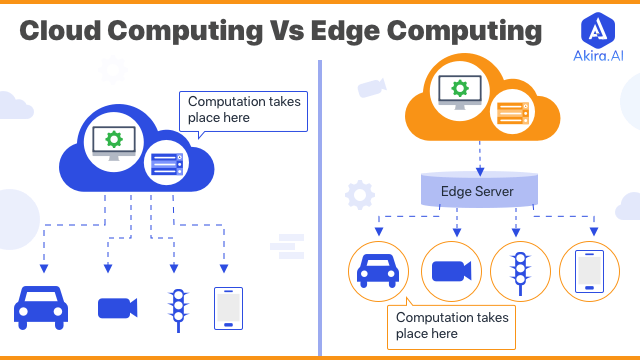
\includegraphics[width=0.9\textwidth]{images/akira-ai-cloud-computing-vs-edge-computing.png}
    \caption{Porovnání architektury a datových toků u~edge a cloudového zpracování (převzato z~\cite{akira_edge_cloud})}
    \label{fig:edge_vs_cloud}
\end{figure}

Na obrázku~\ref{fig:edge_vs_cloud} je schematicky znázorněn rozdíl mezi oběma přístupy. Cloud computing se spoléhá na centrální servery, což vytváří úzké hrdlo na síťové vrstvě. Edge computing naopak přesouvá výpočetní logiku (inferenci) až na samotný okraj sítě k~senzorům, což garantuje vysokou propustnost a okamžité vyhodnocování.

\subsection{Hardwarové AI akcelerátory}
\acs{AI} akcelerátory, často označované jako \acs{NPU} (z~angl. \textit{Neural Processing Unit}), jsou specializované integrované obvody navržené primárně pro efektivní provádění tenzorových výpočtů. Na rozdíl od univerzálních centrálních procesorů (\acs{CPU}) jsou tyto čipy na hardwarové úrovni optimalizovány pro masivní paralelní zpracování maticových operací, jež tvoří matematický základ hlubokých konvolučních sítí.

V~kontextu \acs{Edge AI} jsou tyto akcelerátory naprosto nezbytné, protože překonávají tzv. von Neumannovo úzké hrdlo. Běžné procesory ztrácejí obrovské množství času a energie neustálým přesouváním mezivýsledků mezi výpočetními jednotkami a hlavní pamětí. Akcelerátory tento problém eliminují tím, že udržují data co nejblíže samotným výpočetním jádrům. Umožňují tak nasazení složitých detekčních a sledovacích modelů na energeticky úsporných a prostorově omezených vestavěných zařízeních, a to při zachování propustnosti nutné pro plynulou analýzu dopravy bez závislosti na výkonných serverových farmách~\cite{hailo_alpr_2024, hailo_architecture_2026}.

\subsection{Platforma Raspberry Pi a akcelerace pomocí Hailo-8}
Platforma Raspberry Pi \footnote{\href{https://rpishop.cz}{Rpishop}} představuje rodinu kompaktních jednodeskových počítačů (z~angl. \textit{Single-Board Computers}), které se staly standardem pro prototypování a vývoj vestavěných systémů. Její hlavní vlastností a výhodou je nízká pořizovací cena, obrovská komunitní podpora, stabilní operační systém (založený na linuxovém jádře) a především široká škála hardwarových rozhraní pro připojení periferních senzorů a modulů~\cite{raspberrypi_docs_2024}.

Zásadním omezením samotné architektury Raspberry Pi je však její hrubý výpočetní výkon. Integrovaný procesor postavený na architektuře \acs{ARM} není schopen v~reálném čase zpracovávat náročné úlohy počítačového vidění, a už vůbec ne zajišťovat běh hlubokých neuronových sítí. Z~tohoto důvodu je pro nasazení v~systémech monitorování dopravy nezbytné doplnit základní desku o~externí výpočetní modul~\cite{raspberrypi_ai_kit}.

\begin{figure}[H]
    \centering
    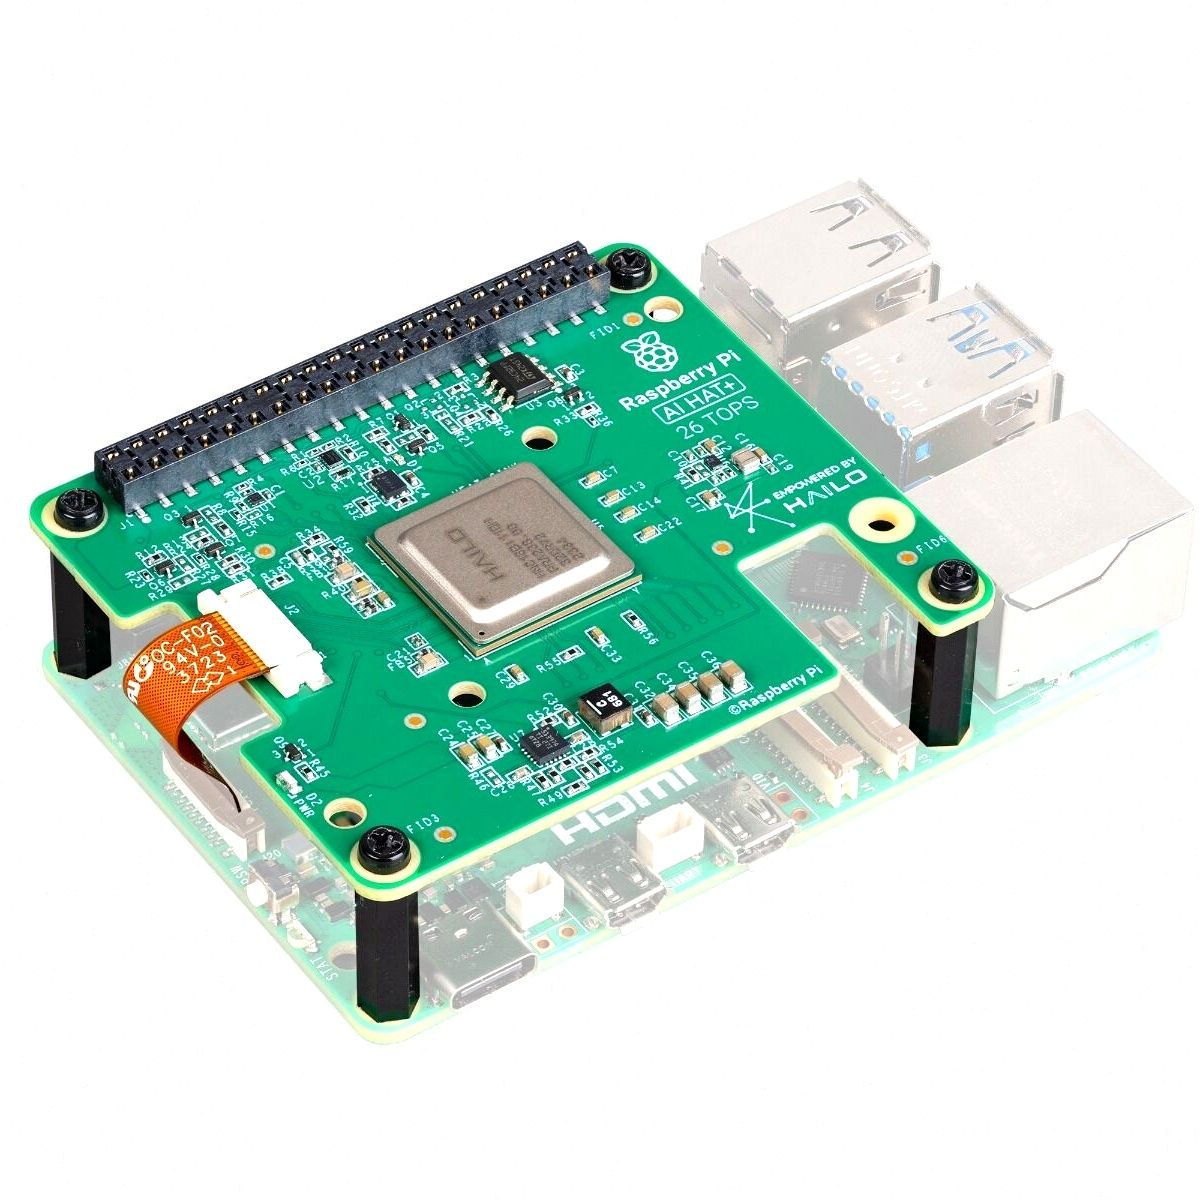
\includegraphics[width=0.75\textwidth]{images/device_with_hailo_processor.jpg}
    \caption{Rozšiřující modul Raspberry Pi AI HAT+ s~integrovaným procesorem Hailo-8 (převzato z~\cite{rpishop_ai_hat})}
    \label{fig:hailo_antratek}
\end{figure}
\vspace{-0.2cm}
Řešením tohoto výpočetního omezení je využití specializovaných rozšiřujících desek, jako je modul Raspberry Pi AI HAT+ (znázorněný na obrázku~\ref{fig:hailo_antratek}). Srdcem tohoto modulu, připojeného přes rozhraní \acs{PCIe}, je pokročilý AI procesor Hailo-8 od stejnojmenné izraelské společnosti, jež se specializuje na vývoj výkonných neurálních akcelerátorů.

Klíčovým parametrem tohoto akcelerátoru je deklarovaný výpočetní výkon 26 TOPS (z~angl. \textit{Tera Operations Per Second}). Předpona „Tera“ v~matematickém vyjádření představuje hodnotu $10^{12}$. Tento čip je tedy fyzicky schopen odbavit masivních $26 \times 10^{12}$ (26 bilionů) operací za jedinou sekundu při inferenci modelu. To, jakým způsobem tohoto výkonu dosahuje, je však stejně důležité jako samotná číselná hodnota. Čipy Hailo využívají inovativní architekturu řízenou datovým tokem (z~angl. \textit{Structure-Defined Dataflow Architecture}). Zatímco tradiční \acs{GPU} zpracovávají vrstvy neuronové sítě sekvenčně a neustále zapisují data do externí paměti, Hailo-8 mapuje celou topologii neuronové sítě přímo na své hardwarové zdroje. Obrazová data tak čipem protékají kontinuálně od jedné vrstvy ke druhé bez nutnosti přístupu k~externí \acs{RAM}.

Tato obrovská výpočetní propustnost spojená s~extrémní energetickou účinností neposkytuje pouze dostatek výkonu pro plynulý běh pokročilých modelů rodiny YOLO. Systému dodává takovou kapacitní rezervu, že dokáže inferenci vysoce paralelizovat. V~praxi to znamená, že systém může přijímat a vyhodnocovat obrazová data z~několika nezávislých video streamů zcela naráz (například synchronní analýza \acs{RTSP} toků ze dvou různých IP kamer na křižovatce), aniž by došlo k~degradaci počtu zpracovaných snímků za sekundu \acs{FPS}~\cite{hailo_alpr_2024, hailo_architecture_2026}. Tím se toto kompaktní hardwarové řešení stává vysoce škálovatelným nástrojem pro robustní a přesné sledování dopravy.

\section{Metodika testování a evaluace}
Vyhodnocení kvality systémů pro detekci, sledování a počítání objektů představuje nedílnou součást návrhu a implementace řešení založených na počítačovém vidění. Cílem evaluace je objektivně posoudit spolehlivost navrženého systému a identifikovat jeho limity. V~oblasti dopravního monitorování je však důležité odlišit hodnocení samotného matematického modelu (zda správně detekuje obdélníky v~izolovaném snímku) od hodnocení celého systému jako funkčního celku (zda spolehlivě počítá vozidla v~čase)~\cite{szeliski_computer_vision, zhou_traffic_survey_2024}.

\subsection{Metodika vyhodnocení detekce v~reálném prostředí}
Pro vyhodnocení přesnosti rozpoznávání objektů nasazeným modelem YOLO v~konkrétním kamerovém streamu se využívá metoda manuální obrazové analýzy vybraných referenčních snímků. Vzhledem k~absenci předem připraveného a anotovaného datasetu pro danou lokaci jsou z~videozáznamu extrahovány reprezentativní statické snímky (např. v~různých světelných podmínkách či při různé hustotě provozu).

V~těchto izolovaných snímcích je následně provedeno pečlivé manuální sečtení a označení všech reálně přítomných vozidel lidským pozorovatelem, čímž vzniká lokální referenční vzorek (\textit{ground truth}). Výstup detekčního modelu na stejném snímku je s~tímto vzorkem vizuálně porovnán, přičemž jsou pro každou třídu identifikovány a zaznamenány následující hodnoty:
\begin{itemize}
    \item \textbf{True Positives (TP):} Správně detekovaná vozidla. Model označil ohraničujícím boxem vozidlo tam, kde se skutečně fyzicky nachází.
    \item \textbf{False Positives (FP):} Falešné detekce. Model označil za vozidlo něco, co ním není (např. stín, značku, sloup), případně vytvořil duplicitní překrývající se detekci pro jedno a to samé auto.
    \item \textbf{False Negatives (FN):} Nerozpoznaná vozidla. Vozidlo na snímku prokazatelně je, ale model jej vůbec nedetekoval.
    \item \textbf{True Negatives (TN):} Správně zamítnuté pozadí. Tento stav označuje prázdný prostor, který model správně ignoroval. V~kontextu detekce objektů ohraničujícími boxy se však hodnota TN v~praxi nepočítá. 
\end{itemize}

Vztah mezi predikcí modelu a skutečností se ve strojovém učení standardně vizualizuje pomocí tzv. matice záměn (z~angl. \textit{Confusion Matrix}), která je pro přehlednost znázorněna v~tabulce~\ref{tab:confusion_matrix_theory}.

\begin{table}[H]
    \centering
    \begin{tabular}{|l|l|l|}
        \hline
        \textbf{Predikce/Skutečnost} & \textbf{Vozidlo je přítomno} & \textbf{Vozidlo není přítomno} \\ \hline
        \textbf{Model hlásí detekci} & TP & FP \\ \hline
        \textbf{Model nehlásí detekci} & FN & TN \\ \hline
    \end{tabular}
    \caption{Základní matice záměn (Confusion Matrix).}
    \label{tab:confusion_matrix_theory}
\end{table}

Na základě těchto hodnot jsou následně vypočítány reálné metriky pro danou scénu. Tato analýza poskytuje kritický vhled do toho, do jaké míry případné chyby ve finálním sčítání pocházejí z~nepřesné primární detekce a do jaké míry jsou způsobeny až selháním sledovacího algoritmu.

\subsection{Metriky hodnocení detekčních modelů}
Při samotném vývoji a trénování detekčních modelů se k~objektivnímu měření výkonu na referenčních datasetech (tzv. \textit{ground truth}) využívá standardizovaná sada matematických metrik~\cite{szeliski_computer_vision}:

\begin{itemize}
    \item \textbf{Precision (Přesnost):} Vyjadřuje podíl skutečně správných detekcí vůči všem detekcím, které model vyprodukoval. Indikuje, jak moc lze věřit modelu, když ohlásí nález vozidla.
    $$ Precision = \frac{TP}{TP + FP} $$
    \item \textbf{Recall (Úplnost):} Udává schopnost systému nalézt všechny relevantní objekty přítomné ve scéně. Definuje se jako podíl správně detekovaných objektů vůči reálnému počtu existujících objektů.
    $$ Recall = \frac{TP}{TP + FN} $$
    \item \textbf{IoU (Intersection over Union):} Vyjadřuje exaktní míru geometrického překryvu mezi predikovaným ohraničujícím boxem ($B_{pred}$) a reálným boxem ($B_{gt}$). Čím více se hodnota blíží k~jedné, tím je lokalizace přesnější.
    $$ IoU = \frac{\text{Plocha průniku}}{\text{Plocha sjednocení}} = \frac{|B_{pred} \cap B_{gt}|}{|B_{pred} \cup B_{gt}|} $$
    \item \textbf{mAP (Mean Average Precision):} Představuje komplexní ukazatel výkonu modelu napříč všemi detekovanými třídami ($N$), který zohledňuje přesnost, úplnost i kvalitu lokalizace zjištěnou pomocí křivky Average Precision ($AP$).
    $$ mAP = \frac{1}{N} \sum_{i=1}^{N} AP_i $$
    \item \textbf{Accuracy (Přesnost klasifikace):} Metrika vyjadřující celkový podíl všech správných rozhodnutí. Jak již bylo zmíněno, v~detekci objektů má vzhledem k~obrovské nerovnováze mezi počtem objektů a plochou prázdného pozadí (obrovské a nedefinovatelné množství TN) jen mizivou vypovídající hodnotu.
    $$ Accuracy = \frac{TP + TN}{TP + TN + FP + FN} $$
\end{itemize}

Vzhledem k~tomu, že v~rámci této bakalářské práce je implementován a nasazován již hotový předtrénovaný model z~rodiny YOLO, není primárním cílem optimalizace jeho interních vah pomocí výše zmíněných metrik na testovacích datasetech. Cílem je naopak ověření jeho reálné propustnosti a praktické výkonnosti jakožto sčítacího softwarového uzlu v~konkrétním dopravním prostředí.

\subsection{Metodika vyhodnocení počítání v~reálném prostředí}
Vyhodnocení správnosti sčítání objektů je v~dopravních aplikacích klíčové. Na rozdíl od detekce izolovaných snímků se zde hodnotí konzistence sledovacího algoritmu (např. zda udrží ID vozidla) a správná prostorová identifikace průjezdů vyhrazenými počítacími liniemi. 

Hlavními zdroji chyb v~reálném prostředí jsou časté vizuální překryvy objektů (okluze), ztráta identifikátoru způsobující opakované započítání téhož vozidla, nebo dynamické změny světelných podmínek a vrhání stínů. Jak potvrzují srovnávací studie zaměřené na reálné nasazení video-detekčních počítacích systémů, právě tyto faktory vnějšího prostředí představují největší výzvu pro udržení vysoké a stabilní provozní přesnosti~\cite{zhou_traffic_survey_2024}, \cite{pronello_2023}.

V~reálném nasazení bez existence předem připravených exaktních datových sad je standardní evaluační metodou vytvoření vlastní sady referenčních dat (tzv. ground truth) formou nezávislého manuálního sčítání z~pořízeného videozáznamu~\cite{mdpi_roi_tracking_2022}, \cite{pronello_2023}. Referenční hodnota je tak získána nezávislým pozorováním, čímž je stanoven skutečný počet průjezdů vozidel ($N_{real}$). Tento údaj je následně porovnán s~počtem vozidel detekovaných automatizovaným systémem ($N_{sys}$) pomocí metriky poměrové přesnosti sčítání ($Accuracy_{count}$):

$$Accuracy_{count} = \left( 1 - \frac{|N_{real} - N_{sys}|}{N_{real}} \right) \cdot 100 \ [\%]$$

Tato metrika věrně a zcela exaktně reflektuje celkovou provozní úspěšnost systému při kontinuálním sčítání vozidel, a právě ona bude využita jako primární hodnoticí ukazatel v~testovací části této práce.

\section{Etické aspekty a GDPR}
Při návrhu, nasazení a provozu jakýchkoliv kamerových systémů na veřejných prostranstvích a dopravních komunikacích je absolutně nezbytné zohlednit principy ochrany osobních údajů. Tyto povinnosti primárně vyplývají z~platného Nařízení Evropského parlamentu a Rady (EU) 2016/679, obecně známého pod zkratkou \acs{GDPR} (z~angl. \textit{General Data Protection Regulation}). Moderní kamerové systémy totiž ze své podstaty mohou neúmyslně zachytávat citlivé identifikační prvky, jakými jsou tváře chodců, řidičů nebo konkrétní registrační značky vozidel.

Navrhované řešení v~rámci této bakalářské práce proto plně a striktně respektuje moderní přístup tzv. \textit{Privacy by Design} (ochrana soukromí již od fáze samotného návrhu softwarové architektury). Tohoto principu je dosaženo právě díky integraci konceptu Edge AI. Veškeré algoritmické zpracování obrazových dat z~kamery probíhá plně lokálně, přímo v~operační paměti okrajového zařízení, které je umístěno bezprostředně u~zdroje videa~\cite{li_edge_ai_2020}. 

Díky lokální a okamžité inferenci se žádný surový obrazový signál, videozáznam ani snímky obsahující potenciální osobní údaje nikam neukládají, neodesílají se přes nezabezpečené sítě a nejsou nahrávány do žádného vzdáleného cloudového úložiště. Do databázového systému se propisují a k~následné vizualizaci odesílají pouze finální, přísně anonymizovaná a agregovaná numerická metadata – například celkový typ objektu (automobil, chodec), hrubý časový údaj, směr jeho pohybu a identifikátor sčítací brány. 

Tento architektonický přístup bezezbytku naplňuje zásadu minimalizace osobních údajů, která je jedním z~nosných a nejdůležitějších pilířů legislativy GDPR. Systém tak poskytuje plnohodnotná statistická data pro analýzu dopravy, aniž by jakýmkoliv způsobem zasahoval do soukromí účastníků provozu.
